
\usetikzlibrary{arrows.meta, positioning}

\begin{figure*}
    \centering

    \label{figure:competence-transfer}
    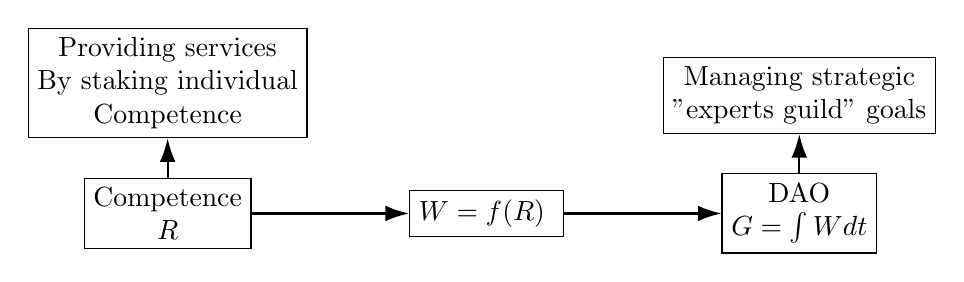
\begin{tikzpicture}[
        node distance=2cm,
        every node/.style={draw, align=center},
        arrow/.style={-{Latex[length=3mm, width=2mm]}, thick}
        ]


        % Single block for the game

        % Nodes
        \node (competence) {Competence \\ $R$};
        % \node[draw, rectangle, minimum width=7.5cm, minimum height=0.5cm, below=of competence] (Game) {r2 g6};
        % Bottom level blocks (5 participants)

        \node (exchange) [right=of competence] { $W = f(R)$  };

        \node (DAO) [right=of exchange] {DAO \\ ${G} = \int{W}dt$ };
        % \node (quorum) [below=of DAO] {Quorum Group \\ $V_{aj}$};
        % \node (dao) [right=of exchange] {DAO \\ $G_j(t)$};
        % \node (market) [below=of DAO] {Market Value \\ Increase};

        % Connect participants to the game
        % \foreach \x in {1,...,5}
        % \draw[->] (P-\x) -- (competence);

        % Arrow pointing upwards from the top block with text "to r3"
        % \draw[->] (Game.north) -- ++(0,1) node[above] {to r3 g31};

        % Arrows
        % \draw [arrow] ()
        \draw [arrow] (competence) -- (exchange);
        \draw [arrow] (exchange) -- (DAO);
        % \draw [arrow] (DAO) -- (quorum);
        % \draw [arrow] (quorum) -- (dao);
        % \draw [arrow] (dao) -- (market);



        % Labels
        \node (Staking)[above=0.5cm of competence] {Providing services \\ By staking individual \\ Competence};
        \draw [arrow] (competence) -- (Staking);
        \node (Managing) [above=0.5cm of DAO] {Managing strategic \\  "experts guild" goals};
        \draw [arrow] (DAO) -- (Managing);
        % \node [above=0.5cm of quorum] {Quorum Group Formation};
        % \node [above=0.5cm of dao] {DAO Representation};
    \end{tikzpicture}
    \caption{Competence transfer to DAO voting weights}

\end{figure*}